\subsection{Functionalities of the Node-RED Application}

Node-RED is a flow-based development tool which was used in this project to implement the backend functionalities, database connectivity, and live dashboards for this project.

\subsubsection{Extracting Data from the Exchange Rate API}

The Exchangeratesapi.io API service has been used to obtain the exchange rates of the selected 6 currency types. The API service used for this application is updated every second with the exchange rates of many types of currencies. For our application we proposed that exchange rates are needed to be sampled at 30 second intervals but a paid account is required with a fee up to USD 80.00 per month to obtain exchange rates at such a high frequency, as shown in the figure.

\begin{figure}[H]
    \centering
      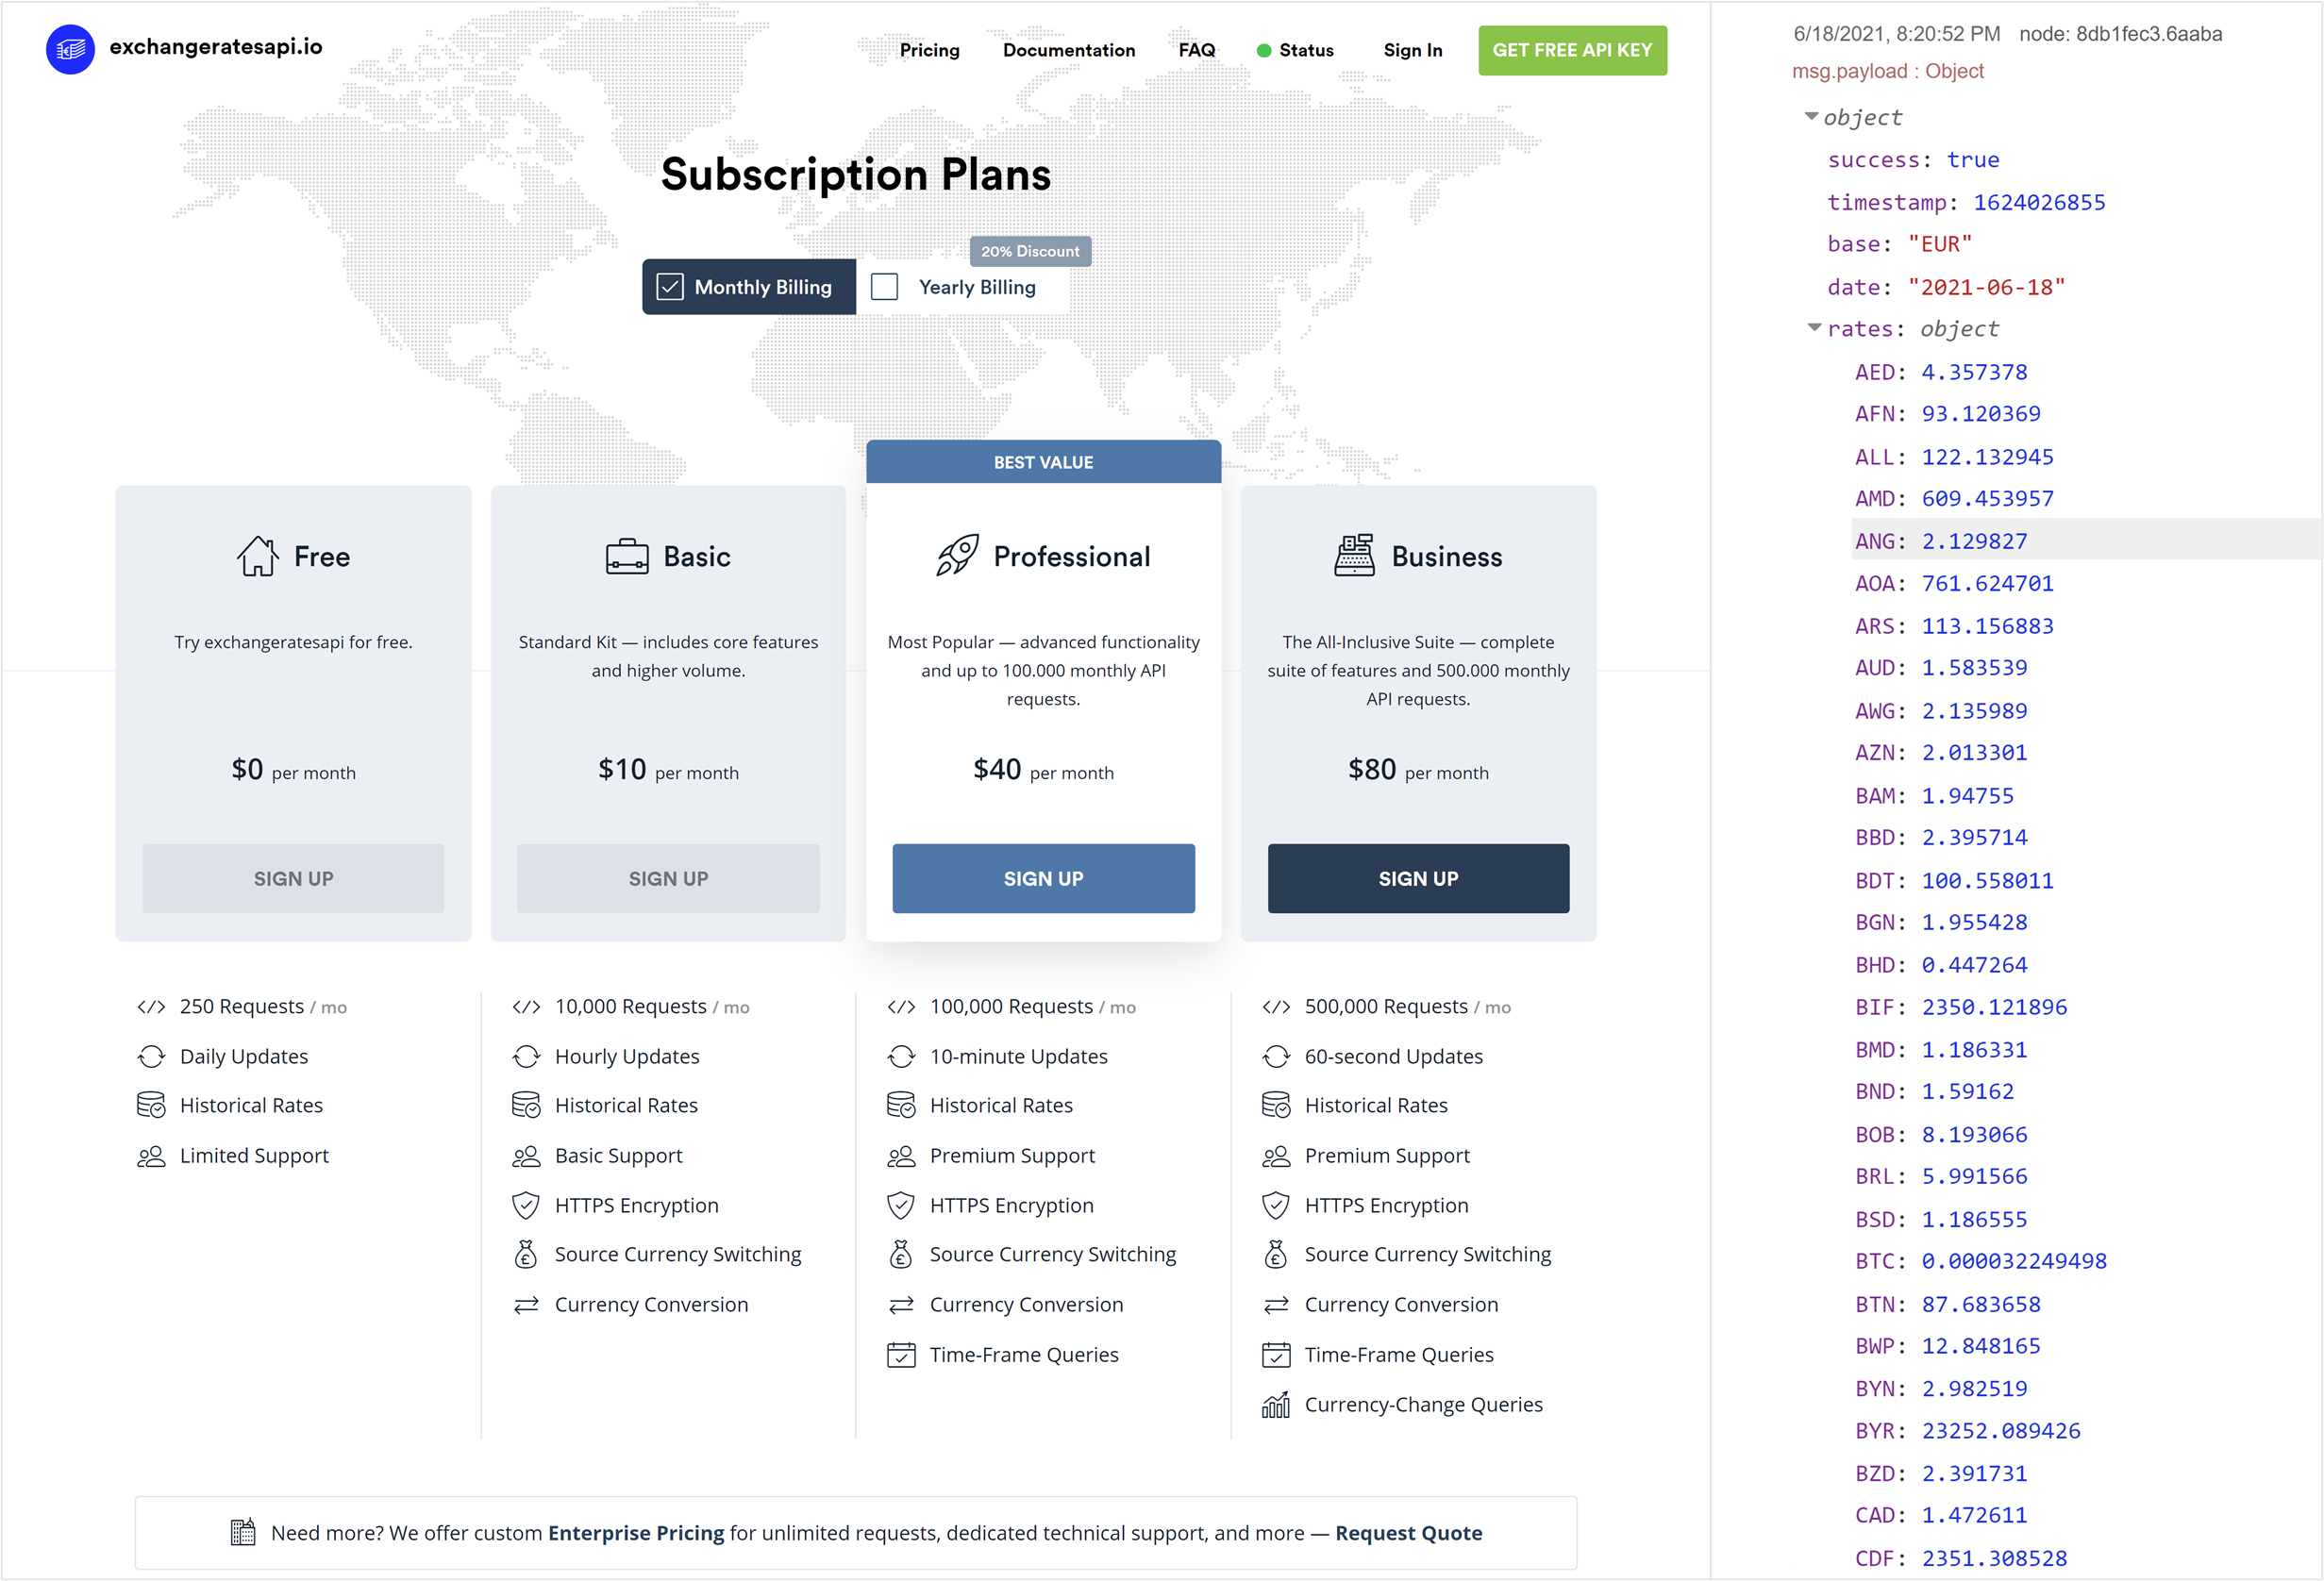
\includegraphics[width=0.8\textwidth]{images/exapi.png}
    \caption{The subscription plans of the API and the Response array containing Exchange rates}
    \label{exapi}
\end{figure}

\begin{figure}[H]
    \centering
      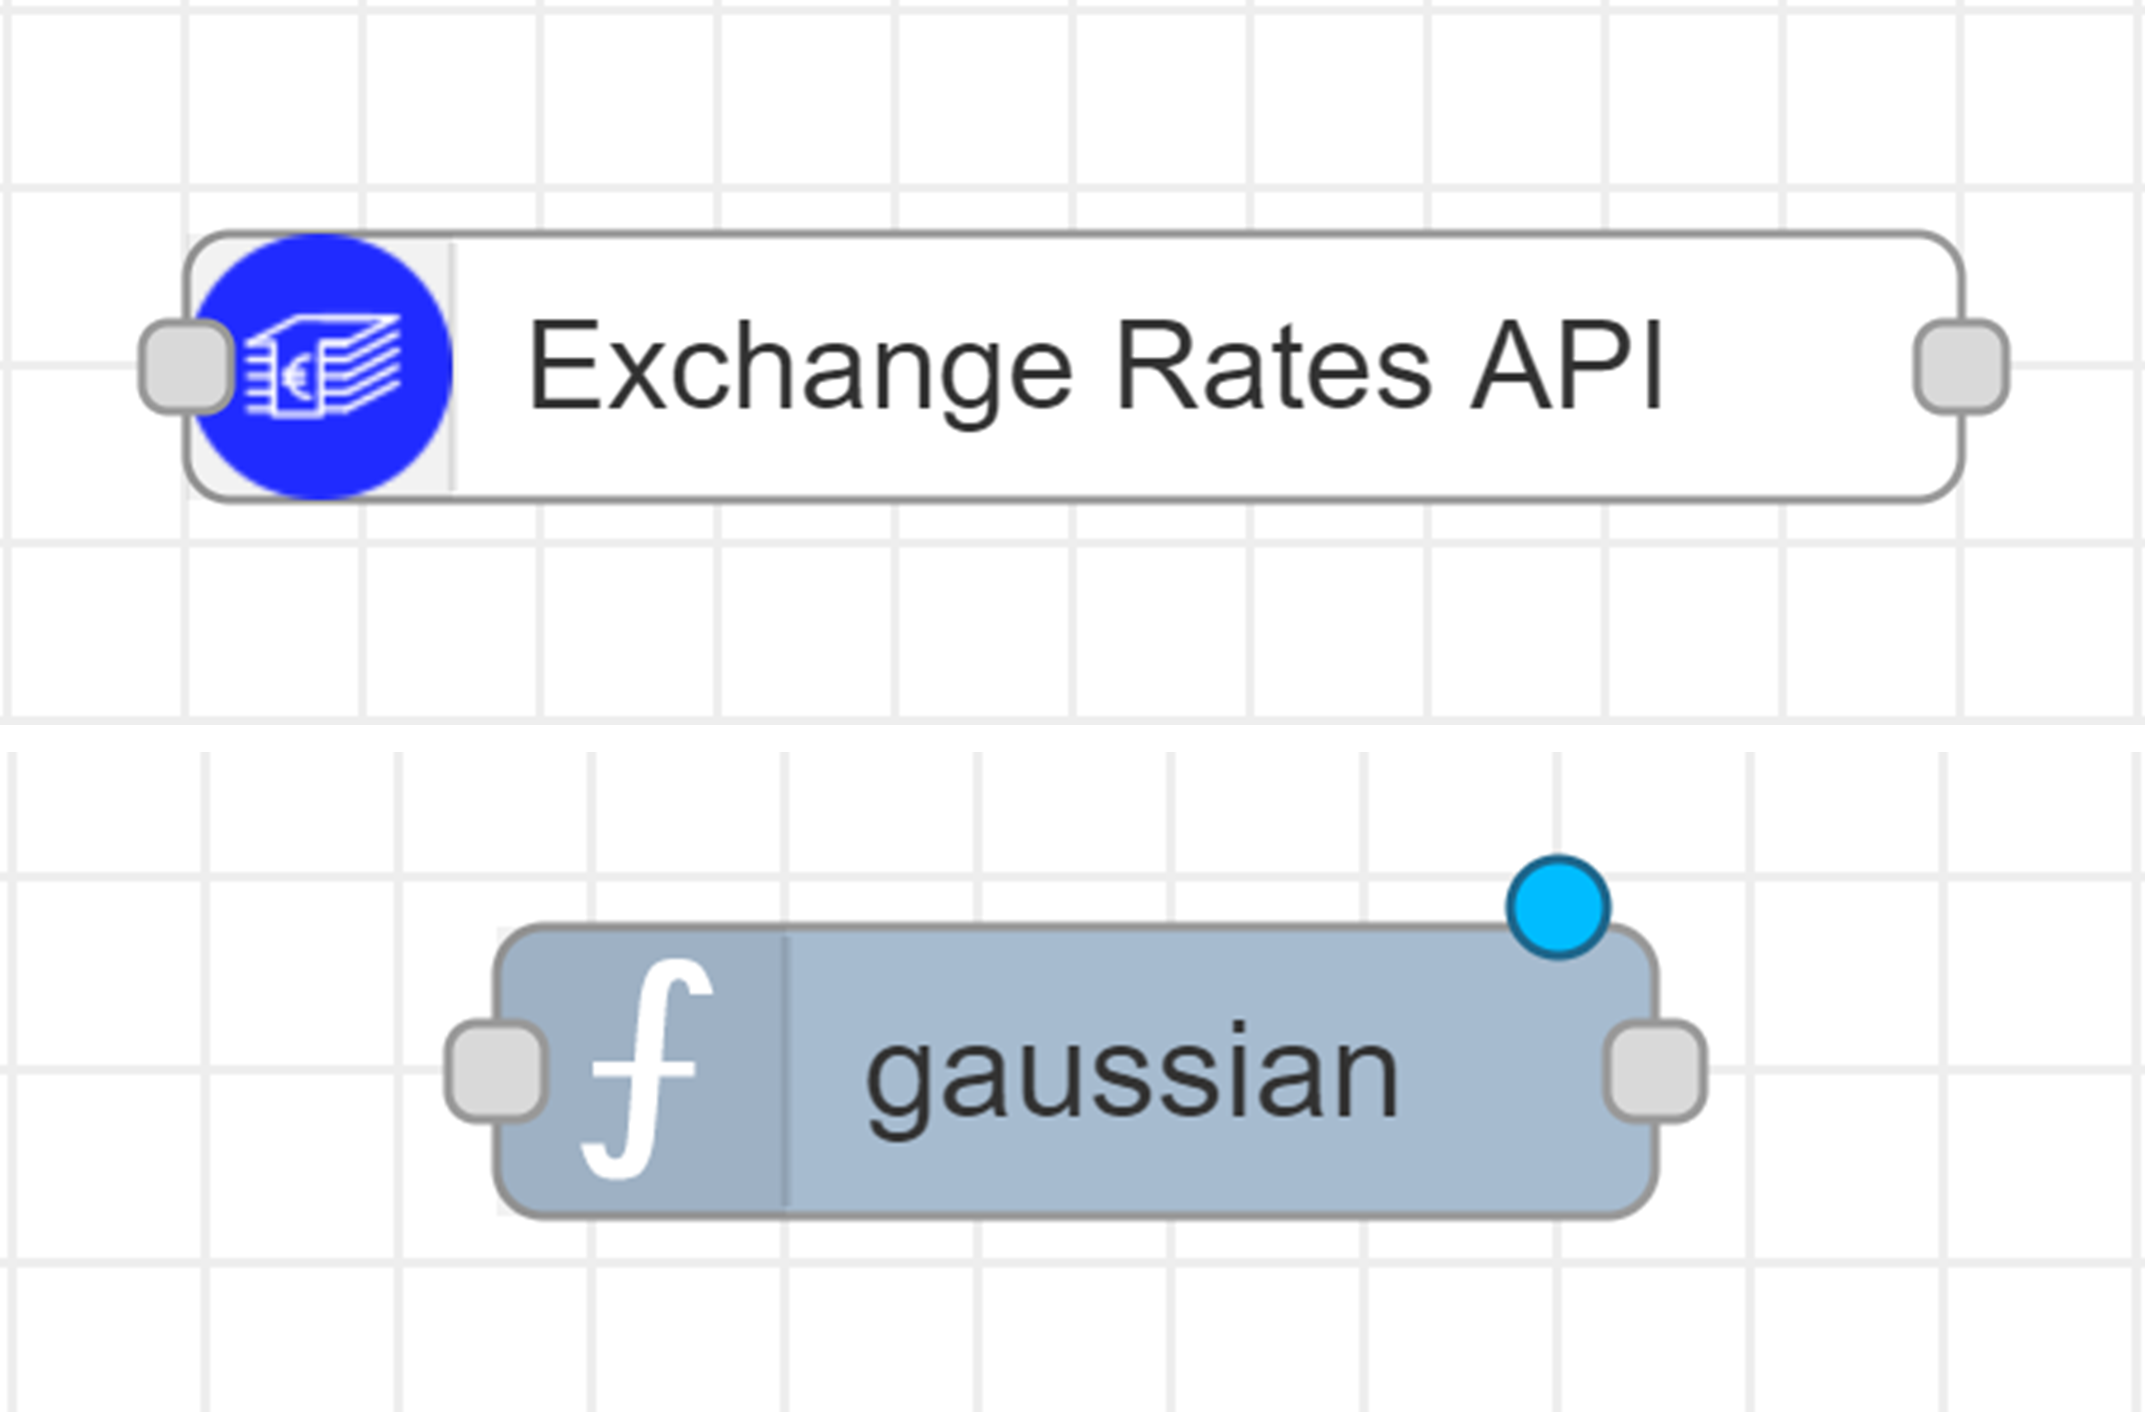
\includegraphics[width=0.4\textwidth]{images/apinodes.png}
    \caption{ Exchange rate API node and Gaussian value generating node}
    \label{exapi}
\end{figure}

Hence, for the purpose of designing a prototype for this application, we have used the free package which updates the exchange rates hourly. Further, we used a random number generator to vary the hourly rate at 30 second intervals so that only its 5th decimal place varies (which is similar to the real variations of exchange rates every 30 seconds) to simulate the actual variation of exchange rates. These were simulated using Node-RED, and the following packages were used.\\

\textbf{a. node-red-contrib-exchangeratesapi \cite{api}}\\

The base currency and the currency of which the exchange rate is required needs to be specified to this node and it sends an API request to retrieve the required exchange rates. The response from this API containing a large collection of exchange rates is shown in figure , from which 6 currency types are selected for our application.\\

A timer was created using the “Inject” node with repeat enabled at hourly intervals to simulate this function.\\

\textbf{b. node-red-contrib-acoustics \cite{acoustics}}\\

The gaussian node from this package (check figure) takes the mean and standard deviation values as inputs and gives a random number as the output. This value was multiplied by the exchange rate in the previous hour and divided by 105to simulate the actual variations of exchange rates every 30 seconds.\\

A timer was created using the “Inject” node with repeat enabled at 30 second intervals to simulate this function.


\subsubsection{Integrating Firebase}

\begin{figure}[H]
    \centering
      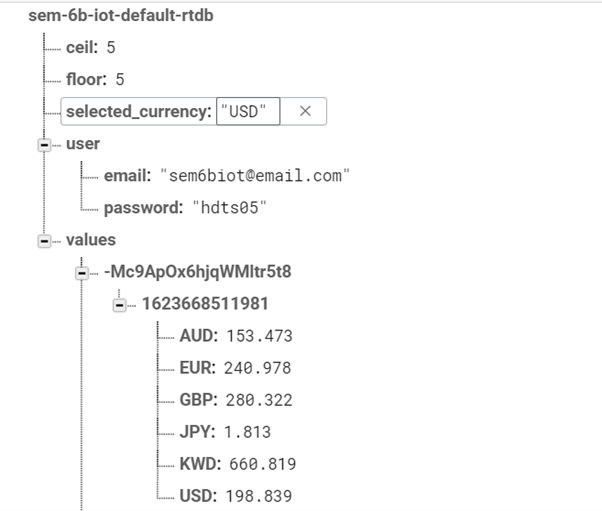
\includegraphics[width=0.6\textwidth]{images/fire.png}
    \caption{Firebase data structure}
    \label{exapi}
\end{figure}

The data obtained hourly through API requests, is stored in a Firebase realtime database \cite{firebase} for future use, as there are no free sources of historical exchange rate data for Day Traders. This functionality was implemented via Node-RED as well using the node-red-contrib-firebase \cite{noderedfire} package.\\

Firebase is able to synchronize data to all its connected clients within milliseconds i.e., any change to the database would be reflected in its applications without the need for HTTP requests. Further, the applications hosted using firebase remain interactive, even when the devices are offline, and synchronizes with the database as soon as connectivity is established.\\

The Firebase realtime database is a cloud-hosted database, and one of the many products and services of Google. This is a NoSQL database and hence the data is stored in JSON format. Figure  shows the structure which was used to store the user data, user ceiling / floor values, and the exchange rates in the Firebase realtime database.\\

Three nodes from the node-red-contrib-firebase package have been used to connect the Firebase Realtime database to the Node-RED application, and they are as follows.\\

\textbf{a. firebase.on}\\

This node listens for changes in the database actively and in realtime and takes any changes to the Node-RED application. This was used to synchronize the ceiling and floor values in the database to the Node-RED application in this project.\\

\textbf{b. firebase.once} \\

This node allows us to read data from the database. This was used to extract the exchange rates over 40 hours when plotting the charts of the Node-RED live dashboard.\\

\textbf{c. firebase.modify}\\

This node is used to write or modify the data in the database using the Node-RED application. This was used when storing the authentication data and exchange rate data in the database.\\

\begin{figure}[H]
    \centering
      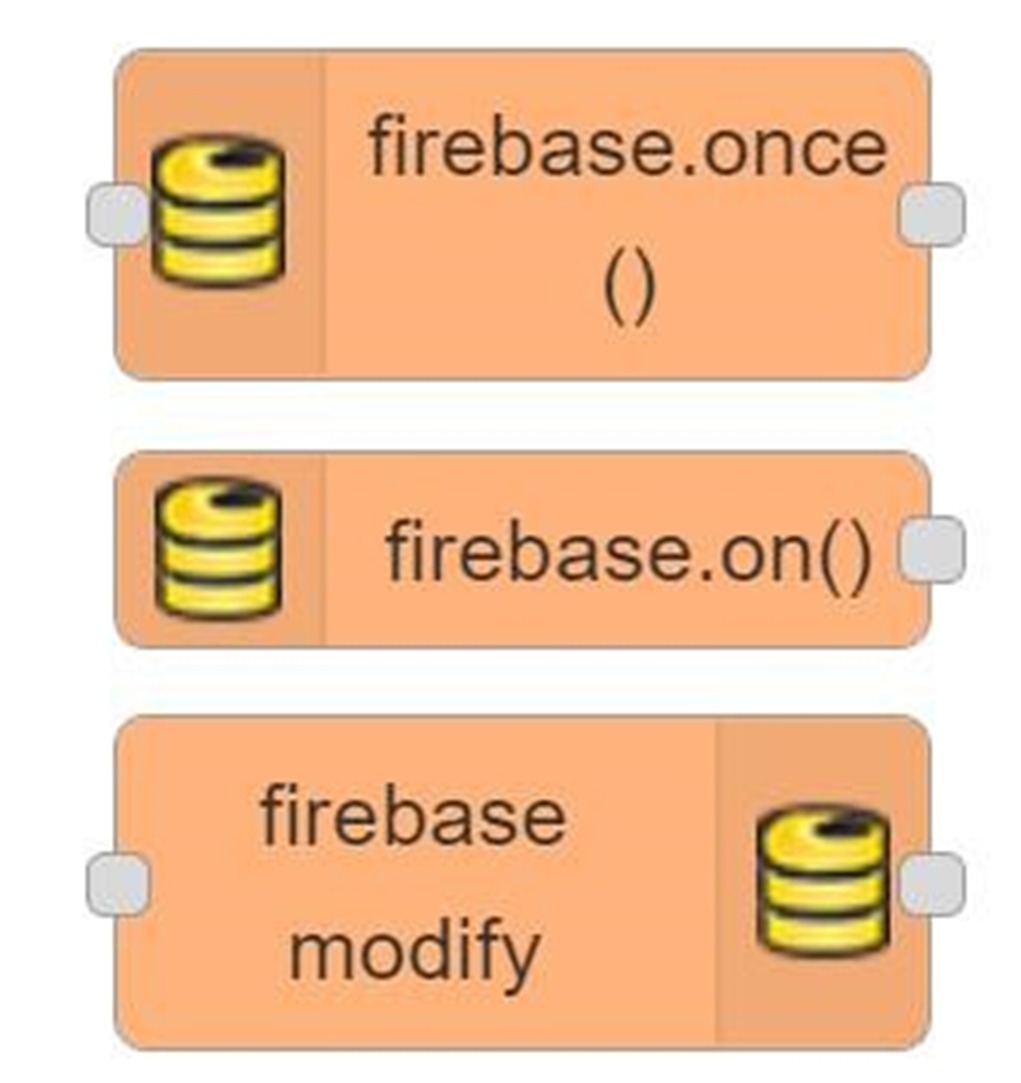
\includegraphics[width=0.4\textwidth]{images/firenodes.png}
    \caption{ Firebase data structure}
    \label{firenodes}
\end{figure}

What we store.

\begin{itemize}[itemsep=-1.7mm]
\item User credentials
\item User inputs : selected currency, ceil, floor
\item Fetched hourly forex values 
\end{itemize}


This is important because the stored data must be available in case of the following situations.

\begin{itemize}[itemsep=-1.7mm]
\item In case nodeMCU resets
\item In case Node-RED server restarts
\item store formatted data into database and fetch from it   
\end{itemize}

\subsubsection{Obtaining technical analysis charts from prices}

The hourly price data collected and stored in the real-time database can be sent through popular technical analysis functions to generate useful charts. These charts can be used to make valuable inferences. To process the price data available, an external library named TechnicalIndicators was used. Using the library, following indicators are calculated for hourly historical currency rates. Each currency will have four technical analysis charts.\\


\begin{enumerate}[itemsep=-1.7mm]
\item \textbf{Moving average lines} are frequently used to smooth the fluctuations in a price chart (or a chart of any time series). A moving average is simply the mean of the last n closing prices.

\item \textbf{Rate of Change oscillator} (ROC) or momentum oscillator is calculated as 100 times the difference between the latest closing price and the closing price n periods earlier. Thus, it oscillates around zero.

\item \textbf{Moving average convergence/divergence} (MACD) oscillators are drawn using exponentially smoothed moving averages, which place greater weight on more recent observations. The “MACD line” is the difference between two exponentially smoothed moving averages of the price.

\item \textbf{Relative Strength Index} (RSI) is based on the ratio of total price increases to total price decreases over a selected number of periods. This ratio is then scaled to oscillate between 0 and 100.
\end{enumerate}

\subsubsection{Creating the Node-RED dashboard}

The exchange rate data obtained from the API were analyzed using Node-RED functions to yield the above values of technical indicators over a period of 40 hours and plotted using a Node-RED dashboard as shown in Fig..

The dashboard contains 6 Tabs, one for each currency type and 4 groups per tab. Each group contains the plot of  a single technical indicator. The Day Trader can predict the future fluctuations of exchange rates by viewing these charts and making decisions on his future investments. If the exchange rates are going to increase in time to come, he would purchase more currency, and if they are to decrease, he would short sell the currency in his possession.
